\section{KKT and Lagrange Duality}

% Basic 2d Example for derivation:
% $\min _{x \in \mathbb{R}^2} f(x)$ s.t. $h(x)=0$
% $\rightarrow$
% $\nabla f(x^\star)$, $\nabla h(x^\star)$
% co-linear
% $\Leftrightarrow$
% $\exists\ \nu^\star \in \mathbb{R}: \nabla f(x^\star)+\nu^\star\nabla h(x^\star) = 0$
% $\Leftrightarrow$
% $f(x)+\nu^\star h(x)$ is stationary at $x^\star$
%
% \subsection{Generalization for $n\rightarrow\infty$ and with constraints}
\vspace{-4mm}
\begin{equation}
	\text{We consider}\
	f^\star = \inf_{x\in\mathcal{\mathbb{R}}^n}f(x)
	\;\text{ s.t. }\ g(x)\le0,h(x)=0
	\label{eq:dual}
\end{equation}
\vspace{-3mm}
$$\begin{aligned}
		                           & \textbf{Lagrange }                                              &
		\mathcal{L}(x,\lambda,\nu) & = f(x) + \lambda\T g(x)+\nu\T h(x)
		\\
		                           & \textbf{Dual Function }                                         &
		d(\lambda,\nu)             & = \inf_{x \in \mathcal{\mathbb{R}}^n}\mathcal{L}(x,\lambda,\nu)
	\end{aligned}$$
\vspace{-2mm}
\begin{proposition}[Weak Duality]
	$d(\lambda,\nu)\le f^\star,\forall\lambda\ge0,\nu\in\mathbb{R}^{h}$
\end{proposition}

\begin{definition}[Constraint  qualification]
	$\mathcal{C}$ convex, \textbf{Slaters Condition} holds if
	$\exists\ \hat{x} \in \mathbb{R}^{n}$ s.t. $h(\hat{x})=0$ and $g(\hat{x})<0$
\end{definition}

\begin{proposition}[Strong Duality]
	If Slater's condition holds
	and (\ref{eq:dual}) is convex
	$\Rightarrow$
	$\exists \lambda \ge 0, \nu \in \mathbb{R}^{n_h}$ s.t. $d(\lambda,\nu)=f^\star$
\end{proposition}

\subsection{KKT (Karush-Kuhn-Tucker) Conditions}

\begin{theorem}[KKT Conditions]
	Slater's condition holds
	and (\ref{eq:dual}) is convex
	$\rightarrow$
	$x^\star \in \mathbb{R}^{n}$ is a minimizer of the primal (\ref{eq:dual})
	and $(\lambda^\star \ge 0,\nu^\star) \in \mathbb{R}^{n_g}\times\mathbb{R}^{n_h}$ is a maximizer of the dual
	$\Leftrightarrow$
	$$\begin{aligned}
			 & \nabla_x\mathcal{L}(x^\star,\lambda^\star,\nu^\star)=0
			 & \text{KKT-1 }
			 & \text{(Stationary Lagrangian)}
			\\
			 & g(x^\star)\le0, h(x^\star)=0
			 & \text{KKT-2 }
			 & \text{(primal feasibility)}
			\\
			 & \lambda^\star\ge0, \nu^\star \in \mathbb{R}^{n_h}
			 & \text{KKT-3 }
			 & \text{(dual feasibility)}
			\\
			 & \lambda^{\star T} g(x^\star)=0=\nu^{\star T} h(x^\star)
			 & \text{KKT-4 }
			 & \text{(compementary slackness)}
			\\
		\end{aligned}$$
	In addition we have:
	$\sup_{\lambda\ge0,\nu\in\mathbb{R}^{n_h}}q(\lambda,\nu)=\inf_{x\in\mathcal{C}}f(x)$
\end{theorem}

\textbf{Remark} Without Slater,
KKT1-4 still implies $x^\star$ minimizes (\ref{eq:dual})
and $\lambda,\nu$ maximizes dual,
but the converse is no longer true.
There can be primal-minimizer/dual-maximizer not satisfy KKT.

\subsection{Subdifferential}

For cv $f$ we have
$f(x)\ge f(\bar{x})+\nabla f(\bar{x})\T(x-\bar{x}),\ \forall x,\bar{x}\in \mathbb{R}^{n}$

\begin{definition}
	$f: \mathbb{R}^{n} \rightarrow \bar{\mathbb{R}}$ cv,
	the \textcolor{hltext}{\hl{ subdifferential of $f$ at $\bar{x}$ }}is:
	$\partial f(\bar{x}):=
		\{\lambda \in \mathbb{R}^{n} \mid
		f(x)\ge f(\bar{x})+\lambda\T(x-\bar{x}),
		\forall x \in \mathbb{R}^{n}
		\}$
	\label{def:subdifferential}
\end{definition}

\begin{proposition}[]
	$f$ (like D\ref{def:subdifferential}),
	$x^\star\in\argmin_x f(x)
		\Leftrightarrow
		0 \in\partial f(x^\star)$
\end{proposition}

\begin{proposition}[Relation to conjugate functions]
	For convex $f$ with $\operatorname{epi}(f)$ closed:
	$y \in \partial f(x) \leftrightarrow x \in \partial f^\star(y)$
\end{proposition}

\begin{flushright}
	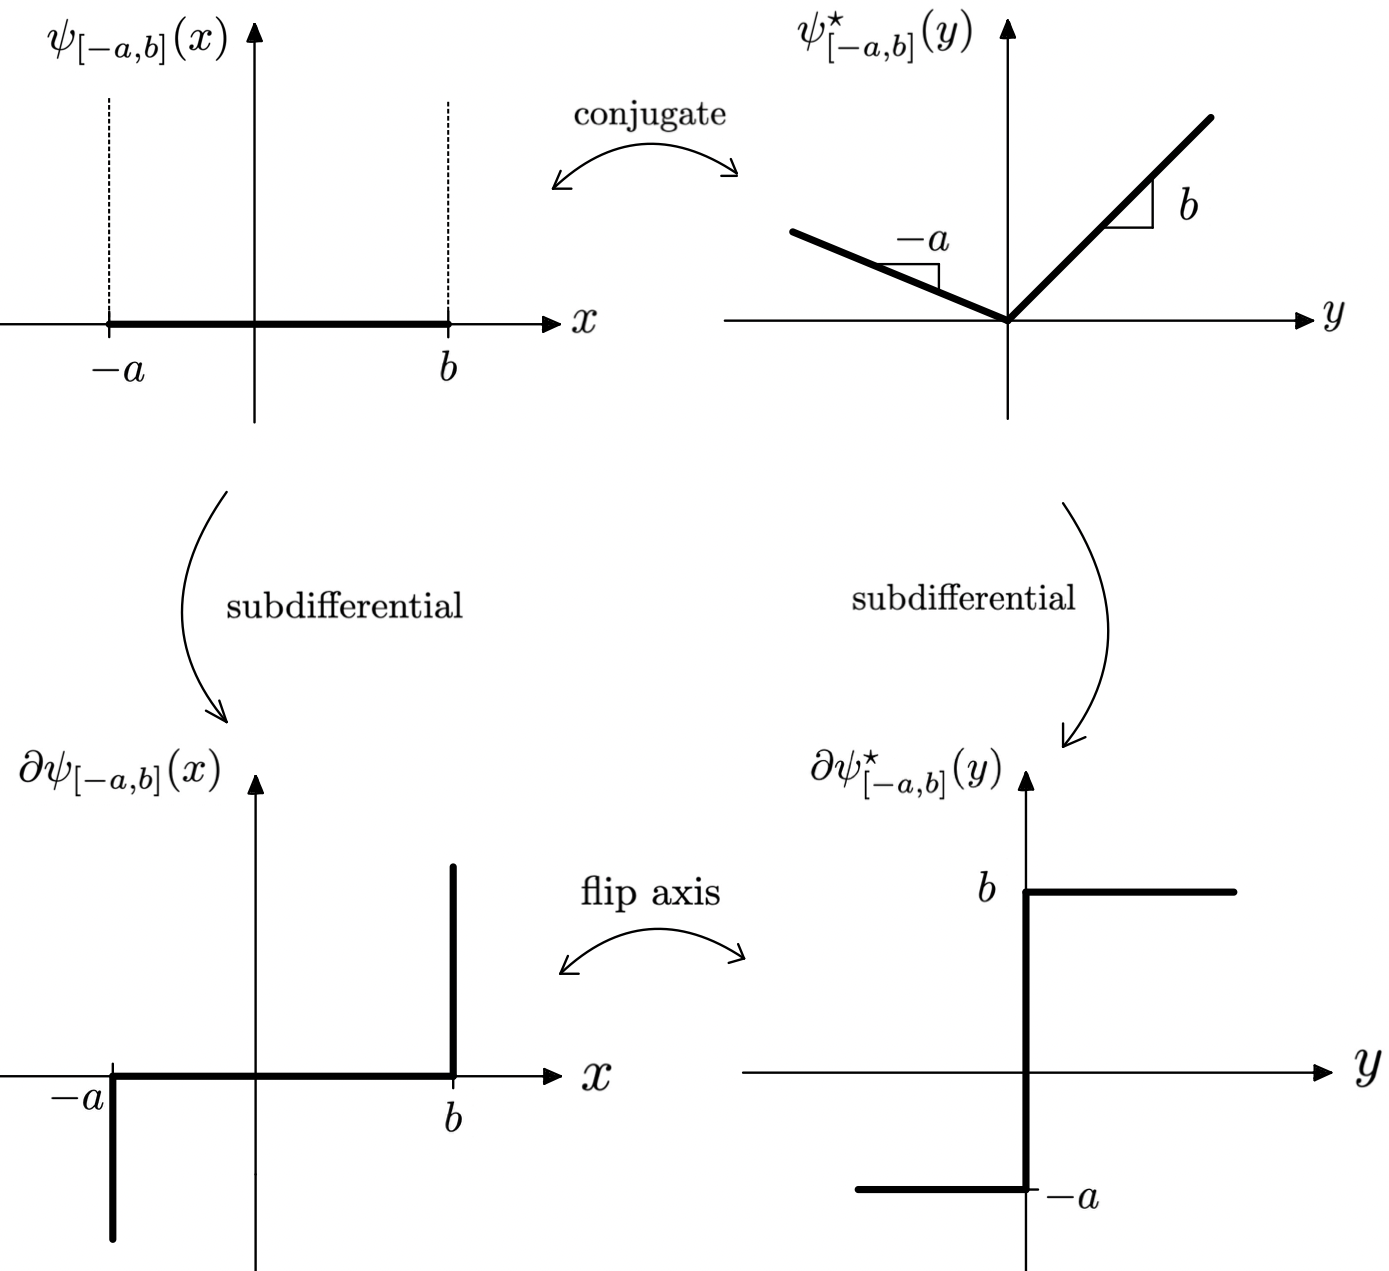
\includegraphics[width=0.92\columnwidth]{images/conjugate_subdiff.png}
\end{flushright}
